%\chapter{開発プロセス}
\section{第4サイクル(10月22日~12月11日)}
第4サイクルは企業講師のビデオ会議が終わった10月22日から12月11日の成果発表会までとした。本サイクルでは、第3サイクルで進めていた実装をさらに進めること、そしてカルタに代わる何か手間のかからない「もの」を提案することを課題として活動を行った。
\par カルタ以外で手間がかからないものは何かを議論した結果、リーフレット\footnote{一枚刷りの印刷物、折りたたみ式の小型の印刷物}という案が生まれた。カルタのように50枚分の印刷をしなければいけないような数による手間をかけず、さらに一枚の紙で作成できて低コストに抑えられるため、この案を採用した。リーフレットの表側には従来の観光パンフレットと同様に木古内の名産等の基本的な観光情報を記し、裏側にはユーザが撮影した写真を自動的に割り当てて独自性のあるものを記せるようにデザイン・実装することにした。しかし、必ずしもユーザがリーフレットを印刷するとも限らないため、アプリ内でも振り返ることができるようにアルバム機能を作ることを決定した。本サイクルで実装した機能は大きく分けて、観光する機能、振り返る機能、そして印刷する機能の3つだ。11月14日にアカデミックリンクがあったため、一旦そこをマイルストーンとして開発し、多くの企業の方や一般の方からレビューを受けた。そのレビューを受けて成果発表会までさらに開発を続けた。具体的に実装した機能・画面は次章で詳説する。前回のサイクルと本サイクルでの主な変化を表5.3に、リーフレットの完成サンプルを図5.7(a)、(b)に示す。アカデミックリンクと成果発表会でのレビュー内容を後に記述する。
\par 本サイクルでは長く続けてきた要件定義が充分に固まったため、比較的実装に集中できて完成度の高いアプリを開発できた。最終報告会での評価も高かったため、今後はプロジェクトが終わっても開発を続けてリリースすることを決定した。そのために、今後は木古内の関係者の方々にキーコ紀行を実際に提案しに行き現地の人のレビューを受けてさらに質の高いアプリにすること、現在残っているバグを取り除くこと、そしてどのように運営していくかを決定することが当面の課題となる。

\begin{table}[htb]
\centering
\addtocounter{table}{+0}
\caption{第3サイクルから第4サイクルへの変化}
  \begin{tabular}{|l|l|} \hline
    改正前&改正後  \\ \hline 
    カルタを作る機能 & \parbox{20zw}{リーフレットを自動生成する機能} \\  \hline
    カルタから思い出を振り返る &\parbox{20zw}{アルバム機能または、リーフレットを用いて思い出を振り返る}\rule[-6mm]{0mm}{14mm}\\ \hline
  \end{tabular} 
\end{table}

\begin{figure}[htbp]
 \begin{center}
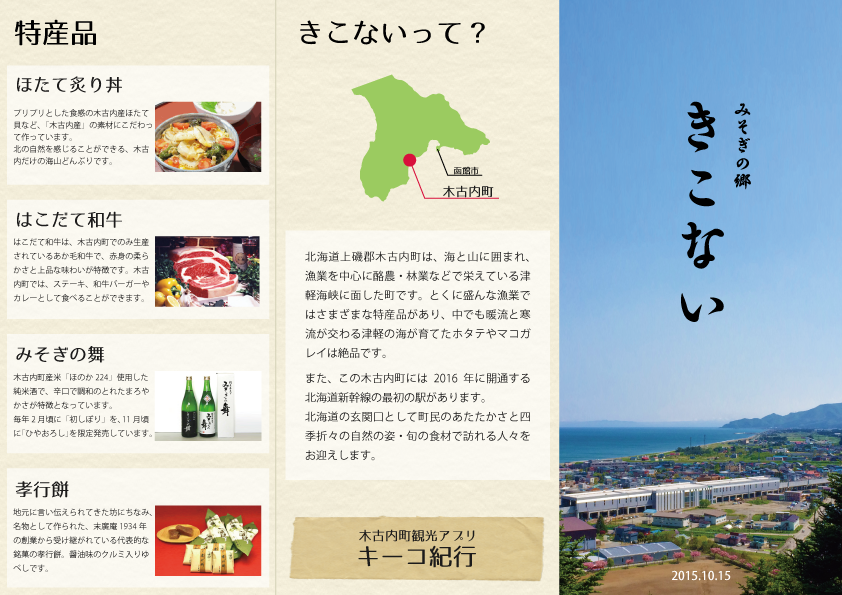
\includegraphics[width=7cm, bb=0 0 857 570]{leaflet_front.png}
 \end{center}
\addtocounter{figure}{+0}
 \caption{(a)リーフレット表側}
 \label{fig:one}
\end{figure}

\begin{figure}[htbp]
 \begin{center}
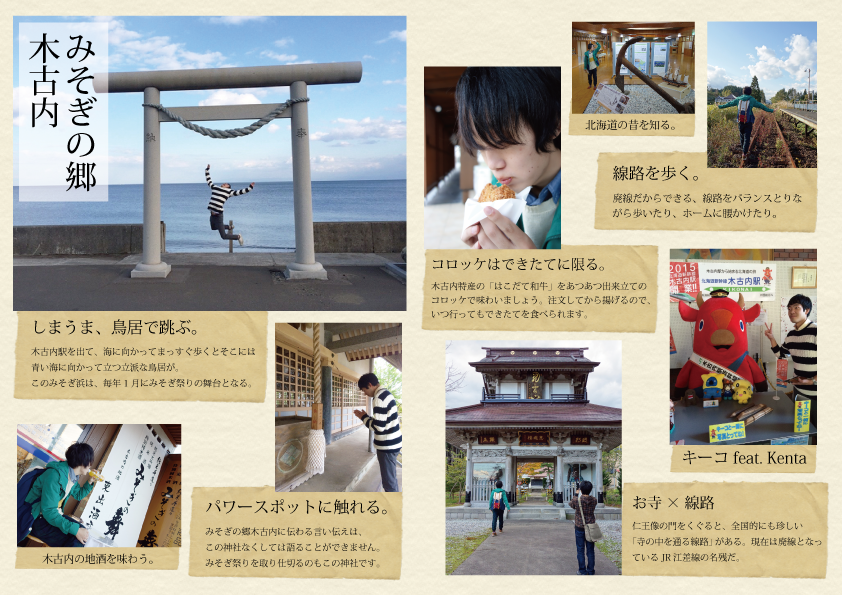
\includegraphics[width=7cm, bb=0 0 857 570]{leaflet_back.png}
 \end{center}
\addtocounter{figure}{-1}
 \caption{(b)リーフレット裏側}
 \label{fig:one}
\end{figure}

\begin{description}
\item[アカデミックリンクでのレビュー内容]\mbox{}
 \begin{itemize}
 \item 継続的に使ってもらう仕組みが足りていない。
 \item フォントが統一されていない。
 \item リーフレットの写真をもう少しまとめてほしい。
 \item ボタンのアイコンや色の配色等、デザイン面をもう少し改善してほしい。
 \end{itemize}
\item[成果発表会でのレビュー内容]\mbox{}
 \begin{itemize}
 \item 利便性とカスタマイズできる点が面白い。
 \item アプリをどうやって広めていくのかがあまりわからなかった。
 \item 自分だけのリーフレットを作れるのは面白い。
 \item 拡張の可能性を感じる。
 \item もっと木古内らしさを出してほしい。
 \item リーフレット作ってもゴミになってしまうのでは。
 \item 操作説明が欲しい。
 \item 検索機能が欲しい。
 \item データではなくものにできるのは良い。
 \item UIデザインが分かりやすい。
 \item 観光情報が分かりやすくまとまっている。
 \item 写真が無駄にならなくて済む。
 \end{itemize}
\end{description}

\bunseki{山川拓也}